%!TEX root = /Users/louis/Documents/PhD/Deliverables/Thesis/thesis.tex

\section{Evaluating Co-evolution Tools}
\label{sec:collaborative_comparison}
This section assesses the extent to which Epsilon Flock (Section~\ref{sec:flock}) can be used for automating developer-driven co-evolution. To this end, Flock is compared to three further co-evolution tools. The comparison identified strengths and weaknesses of the co-evolution tools, and led to the synthesis of a set of recommendations for selecting a co-evolution tool. While Chapter~\ref{Analysis} highlighted theoretical differences between co-evolution tools, this section explores the way in which migration tools compare in practice.

Flock, introduced in Section~\ref{sec:flock}, is a transformation language tailored for model migration. One aspect of the language, conciseness, was evaluated in Section~\ref{sec:quantitive}, and the evaluation performed in this section compares manual specification of model migration in Flock, with three further approaches to automating co-evolution. The results of the comparison, described in Section~\ref{sec:discussion}, suggest situations in which using Flock leads to increased productivity and understandability of model migration, and, conversely, situations in which the other co-evolution tools provide benefits over using Flock. Additionally, the comparison and guidance presented in this section aim to simplify tool selection by recommending tools for particular situations or requirements. The advice presented in this section recommends tools that are suitable, for example, when scalability is a concern (many large models are to be migrated).

The way in which Flock impacts productivity and understandability of model migration might have been explored using a comprehensive user-study, involving hundreds of users. However, locating a large number of participants with expertise in model-driven engineering was not possible given the time constraints of the research. Alternatively, Flock and several further co-evolution tools might have been applied, by the author, to a large, independent co-evolution example in a case study. However, exploring the variations in productivity and understandability of the co-evolution tools would likely have been challenging as the author is obviously more familiar with Flock than the other tools. Instead, the comparison of co-evolution tools was performed using an expert evaluation. Flock and three further co-evolution tools, selected from those described in Chapter~\ref{Analysis}, were compared by MDE experts.

The remainder of this section describes the comparison method, reports results and tool selection guidance, and discusses the situations in which Flock was identified as stronger or weaker than the other co-evolution tools. Section~\ref{sec:method} describes the way in which the co-evolution tools were selected, comparison criteria were identified and the way in which the tools were applied to two co-evolution examples. The experts' experiences with each tool are reported in Section~\ref{sec:results}. Section~\ref{sec:discussion} presents the experts' guidance for identifying the most appropriate model migration tool in different situations, and the section concludes with a description of the strengths and weaknesses of Flock.

\begin{framed}
This section is based on joint work with Markus Herrmannsd\"{o}erfer (a research student at Technische Universit\"at M\"unchen), James Williams (a research student in this department), Dimitrios Kolovos (a lecturer in this department) and Kelly Garc\'{e}s (a research student at EMN-INRIA / LINA-INRIA in Nantes), and has been published in \cite{rose10comparison}. Garc\'{e}s provided assistance with installing and configuration one of the migration tools, and commented on a draft of the paper. Herrmannsd\"{o}erfer, Williams and Kolovos played a larger role in the comparison. Here, the work is narrated to make clear their contributions.
\end{framed}

\subsection{Comparison Method}
\label{sec:method}

\newcommand{\mm}[1]{\texttt{#1}}
The comparison described in this section is based on practical application of the tools to the co-evolution examples described below. This section also discusses the tool selection and comparison processes. Herrmannsd\"{o}erfer and the author identified the co-evolution examples, and formulated the comparison process.

\subsubsection{Co-Evolution Examples}
\label{subsec:method_examples}
To compare migration tools, two examples of co-evolution were used. The first, Petri nets, is a well-known problem in the model migration literature and was used to test the installation and configuration of the migration tools. The second, GMF, is a larger example taken from a real-world model-driven development project, and was identified as a potentially useful example for co-evolution case studies in Chapter~\ref{Analysis} and in \cite{herrmannsdoerfer09gmf}.

\paragraph{Petri Nets.}
The first example is an evolution of a Petri net metamodel, previously used to describe the implementation of Flock in Section~\ref{sec:flock}, and in \cite{cicchetti08automating,garces09managing,wachsmuth07metamodel} to discuss co-evolution and model migration.

\begin{figure}[htbp]
	\centering
	\subfigure[Original metamodel.]
	{
	    \label{fig:petri_nets_original_mm_repeated}
	    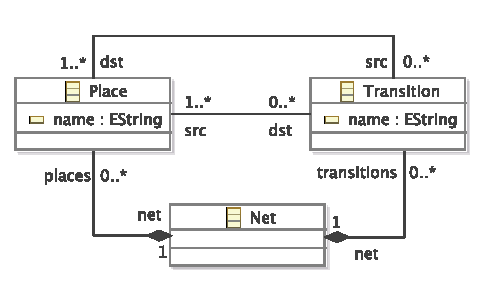
\includegraphics[width=4.75cm]{5.Implementation/images/petri_nets_before.pdf}
	}
	\subfigure[Evolved metamodel.]
	{
	    \label{fig:petri_nets_evolved_mm_repeated}
	    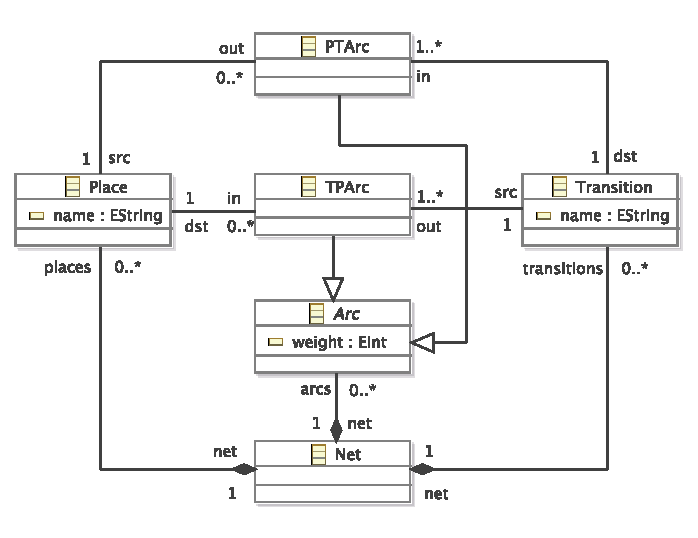
\includegraphics[width=6.25cm]{5.Implementation/images/petri_nets_after.pdf}
	}
	\caption[Exemplar metamodel evolution (Petri nets)]{Petri nets metamodel evolution (taken from \cite{rose10flock}).}
\label{fig:petri_nets_mms_repeated}
\end{figure}

In Figure~\ref{fig:petri_nets_original_mm_repeated}, a Petri \mm{Net} comprises \mm{Place}s and \mm{Transition}s. A \mm{Place} has any number of \mm{src} or \mm{dst} \mm{Transition}s. Similarly, a \mm{Transition} has at least one \mm{src} and \mm{dst} \mm{Place}. In this example, the metamodel in Figure~\ref{fig:petri_nets_original_mm_repeated} is evolved to support weighted connections between \mm{Place}s and \mm{Transition}s and between \mm{Transition}s and \mm{Place}s.

The evolved metamodel is shown in Figure~\ref{fig:petri_nets_evolved_mm_repeated}. \mm{Place}s are connected to \mm{Transition}s via instances of \mm{PTArc}. Likewise, \mm{Transition}s are connected to \mm{Place}s via \mm{TPArc}. Both \mm{PTArc} and \mm{TPArc} inherit from \mm{Arc}, and therefore can be used to specify a \mm{weight}.

\paragraph{GMF.}
The second example is taken from GMF \cite{gronback09emp}, an Eclipse project for generating graphical editors for models. The development of GMF is model-driven and utilises four domain-specific metamodels. Here, we consider one of those metamodels, GMF Graph, and its evolution between GMF versions 1.0 and 2.0. The GMF Graph example is now summarised, and more details can be found in Section~\ref{subsec:gmf_graph}.

\begin{figure}[htbp]
	\centering
	\subfigure[Original metamodel.]
	{
	    \label{fig:gmf_graph_mm_original}
	    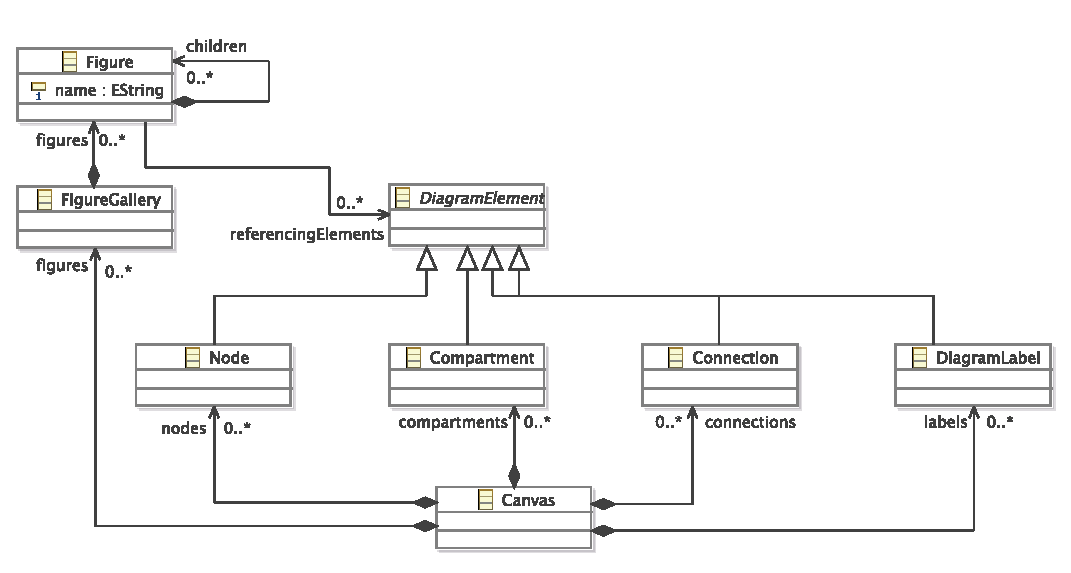
\includegraphics[width=10cm]{A.3.MigrationStrategies/images/gmf/graph_before.pdf}
	}
	\subfigure[Evolved metamodel.]
	{
	    \label{fig:gmf_graph_mm_evolved}
	    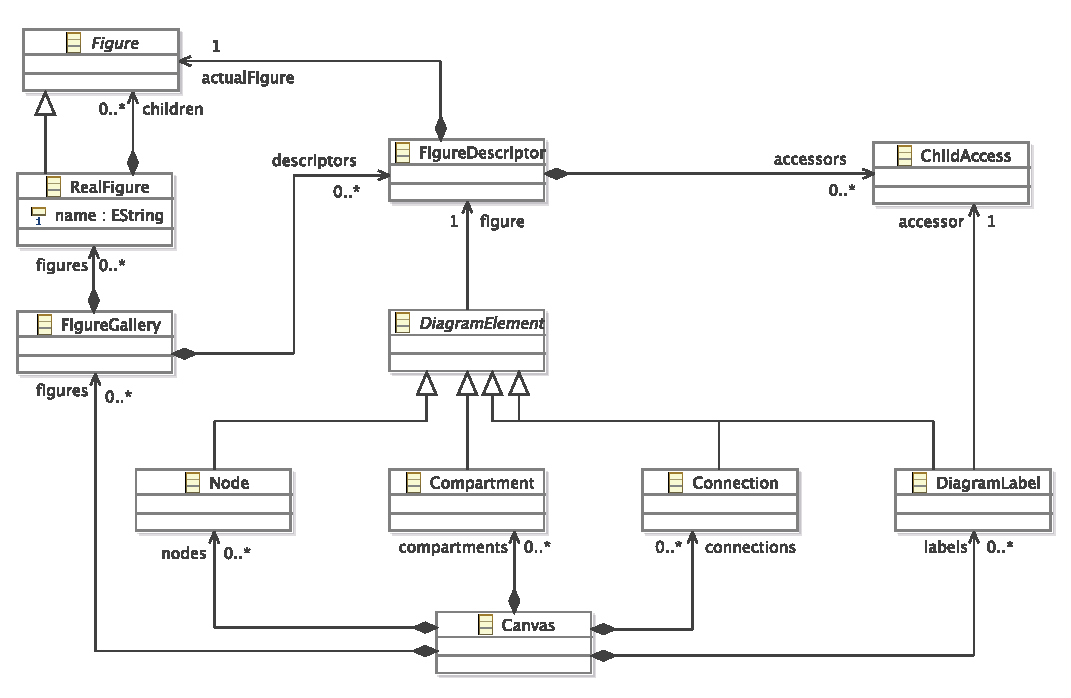
\includegraphics[width=10cm]{A.3.MigrationStrategies/images/gmf/graph_after.pdf}
	}
	\caption{GMF graph metamodel evolution}
\label{fig:gmf_graph_mms}
\end{figure}

The GMF Graph metamodel (Figure~\ref{fig:gmf_graph_mms}) describes the appearance of the generated graphical model editor. As described in the GMF Graph documentation\footnote{\url{http://wiki.eclipse.org/GMFGraph_Hints}}, the Graph metamodel from GMF 1.0 was evolved -- as shown in Figure~\ref{fig:gmf_graph_mm_evolved} -- to facilitate greater re-use of figures by introducing a proxy~\cite{gamma95patterns} for \mm{Fi\-gu\-re}, termed \mm{Fi\-gu\-reDe\-sc\-ri\-pt\-or}. The original \mm{re\-fe\-re\-nc\-in\-gEl\-em\-en\-ts} reference was removed, and an extra metaclass, \mm{Ch\-il\-dAc\-ce\-ss} in its place. Section~\ref{subsec:gmf_graph} discusses the metamodel changes in more detail.

GMF provides a migrating algorithm that produces a model conforming to the evolved Graph metamodel from a model conforming to the original Graph metamodel. In GMF, migration is implemented using Java. The GMF source code includes two example editors, for which the source code management system contains versions conforming to GMF 1.0 and GMF 2.0. For the comparison of migration tools described in this paper, the migrating algorithm and example editors provided by GMF were used to determine the correctness of the migration strategies produced by using each model migration tool.

\subsubsection{Compared Tools}
\label{subsec:method_tools}
The comparison described in this section included one tool from each of the three categories identified in Chapter~\ref{Analysis} -- \emph{manual specification}, \emph{operator-based} and \emph{metamodel matching} approaches. The tools selected were Epsilon Flock, COPE \cite{herrmannsdoerfer09cope} and the AtlanMod Matching Language (AML) \cite{garces09managing}, respectively. A further tool from the manual specification category, Ecore2Ecore, was included because it is distributed with the Eclipse Modeling Framework (EMF), arguably the most widely used modelling framework. AML, COPE and Ecore2Ecore were discussed in Chapter~\ref{Analysis}, and Epsilon Flock in Chapter~\ref{Implementation}.


\subsubsection{Comparison Process}
\label{subsec:method_process}
The comparison of migration tools was conducted by applying each of the four tools (Ecore2Ecore, AML, COPE and Flock) to the two examples of co-evolution (Petri nets and GMF). The developers of each tool were invited to participate in the comparison. The authors of COPE and Flock were able to participate fully, while the authors of Ecore2Ecore and AML were available for guidance, advice, and to comment on preliminary results.

Each tool developer was assigned a migration tool to apply to the two co-evolution examples. Because the authors of Ecore2Ecore and AML were not able to participate fully in the comparison, two colleagues experienced in model transformation and migration, James Williams and Dimitrios Kolovos, stood in. To improve the validity of the comparison, each tool was used by someone other than its developer. Other than this restriction, the tools were allocated arbitrarily.

The comparison was conducted in three phases. In the first phase, criteria against which the tools would be compared were identified by discussion between the tool developers. In the second phase, the first example of co-evolution (Petri nets) was used for familiarisation with the migration tools and to assess the suitability of the comparison criteria. In the third phase, the tools were applied to the larger example of co-evolution (GMF) and results were drawn from the experiences of the tool developers. Table~\ref{tab:criteria} summarises the comparison criteria used, which provide a foundation for future comparisons. The next section presents, for each criterion, observations from applying the migration tools to the co-evolution examples.

\begin{table}[hbtp]
	\centering
	\begin{tabular}{|p{3cm}|p{9cm}|}
	\hline
	\textbf{Name}    & \textbf{Description} \\
	\hline
	Construction     & Ways in which tool supports the development of migration strategies \\
	\hline
	Change           & Ways in which tool supports change to migration strategies \\
	\hline
	Extensibility    & Extent to which user-defined extensions are supported \\
	\hline
	Re-use           & Mechanisms for re-using migration patterns and logic \\
	\hline
	Conciseness      & Size of migration strategies produced with tool \\
	\hline
	Clarity          & Understandability of migration strategies produced with tool \\
	\hline
	Expressiveness   & Extent to which migration problems can be codified with tool \\
	\hline
	Interoperability & Technical dependencies and procedural assumptions of tool \\
	\hline
	Performance      & Time taken to execute migration \\
	\hline
	\end{tabular}
	\label{tab:criteria}
	\caption{Summary of comparison criteria.}
\end{table}


\subsection{Comparison Results}
\label{sec:results}
This section reports the similarities and differences of each tool, using the nine criteria described above. The migration strategies formulated with each tool are available online\footnote{\url{http://github.com/louismrose/migration_comparison}}. 

Each subsection below considers one criterion. This section reports the experiences of the developer to which each tool was allocated. As such, this section contains the work of others. Specifically, Herrmannsd\"{o}erfer described Epsilon Flock, Williams described COPE and Kolovos described Ecore2Ecore. (The author described AML, and introduced each criterion). 

\subsubsection{Constructing the migration strategy}
\label{subsec:constructing}
Facilitating the specification and execution of migration strategies is the primary function of model migration tools. This section reports the process for and challenges faced in constructing migration strategies with each tool.

\paragraph{AML.} An AML user specifies a combination of match heuristics from which AML infers a migrating transformation by comparing original and evolved metamodels. Matching strategies are written in a textual syntax, which AML compiles to produce an executable workflow. The workflow is invoked to generate the migrating transformation, codified in the Atlas Transformation Language (ATL) \cite{jouault05transforming}.
%
Devising correct matching strategies was difficult, as AML lacks documentation that describes the input, output and effects of each heuristic. Papers describing AML (such as \cite{garces09managing}) discuss each heuristic, but mostly in a high-level manner. A semantically invalid combination of heuristics can cause a runtime error, while an incorrect combination results in the generation of an incorrect migration transformation. However, once a matching strategy is specified, it can be re-used for similar cases of metamodel evolution. To devise the matching strategies used in this paper, AML's author provided considerable guidance.

\paragraph{COPE.} A COPE user applies \emph{coupled operations} to the original metamodel to form the evolved metamodel. Each coupled operation specifies a metamodel evolution along with a corresponding fragment of the model migration strategy. A history of applied operations is later used to generate a complete migration strategy.
%
As COPE is meant for co-evolution of models and metamodels, reverse engineering a large metamodel can be difficult. Determining which sequence of operations will produce a correct migration is not always straightforward. To aid the user, COPE allows operations to be undone.
%
To help with the migration process, COPE offers the \emph{Convergence View} which utilises EMF Compare to display the differences between two metamodels. While this was useful, it can, understandably, only provide a list of explicit differences and not the semantics of a metamodel change. Consequently, reverse-engineering a large and unfamiliar metamodel is challenging, and migration for the GMF Graph example could only be completed with considerable guidance from the author of COPE. % For example, it may say that one reference's name and type has changed, but in actual fact a reference class was introduced. This meant that on the larger GMF example, an unfamiliar metamodel, it was difficult to determine exactly what changes needed to be made. Of course, this would be less of a challenge for the author of the metamodel, who has an understanding of how it evolved.

\paragraph{Ecore2Ecore.} In Ecore2Ecore model migration is specified in two steps. In the first step, a graphical mapping editor is used to construct a model that declares basic migrations. In this step only very simple migrations such as class and feature renaming can be declared. In the next step, the developer needs to use Java to specify a customised parser (resource handler, in EMF terminology) that can parse models that conform to the original metamodel and migrate them so that they conform to the new metamodel. This customised parser exploits the basic migration information specified in the first step and delegates any changes that it cannot recognise to a particular Java method in the parser for the developer to handle. Handling such changes is tedious as the developer is only provided with the string contents of the unrecognised features and then needs to use low-level techniques -- such as data-type checking and conversion, string splitting and concatenation -- to address them. Here it is worth mentioning that Ecore2Ecore cannot handle all migration scenarios and is limited to cases where only a certain degree of structural change has been introduced between the original and the evolved metamodel. For cases which Ecore2Ecore cannot handle, developers need to specify a custom parser without any support for automated element copying.

\paragraph{Flock.} In Flock, model migration is specified manually. Flock automatically copies only those model elements which still conform to the evolved metamodel. Hence, the user specifies migration only for model elements which no longer conform to the evolved metamodel.
%
Due to the automatic copying algorithm, an empty Flock migration strategy always yields a model conforming to the evolved metamodel. Consequently, a user typically starts with an empty migration strategy and iteratively refines it to migrate non-conforming elements. However, there is no support to ensure that all non-conforming elements are migrated. In the GMF Graph example, completeness could only be ensured by testing with numerous models.
%
Using this method, a migration strategy can be easily encoded for the Petri net example. For the GMF Graph example whose metamodels are larger, it was more difficult, since there is no tool support for analysing the changes between original and evolved metamodel. %to show how to correctly use the elements of original and evolved metamodel. It is necessary to open editors for both metamodel versions and switch between the strategy editor and these editors back and forth.

\subsubsection{Changing the migration strategy}
Migration strategies can change in at least two ways. Firstly, as a migration strategy is developed, testing might reveal errors which need to be corrected. Secondly, further metamodel changes might require changes to an existing migration strategy.

\paragraph{AML.}  Because AML automatically generates migrating transformations, changing the transformation, for example after discovering an error in the matching strategy, is trivial. To migrate models over several versions of a metamodel at once, the migrating transformations generated by AML can be composed by the user. AML provides no tool support for composing transformations.

\paragraph{COPE.} As mentioned previously, COPE provides an undo feature,
% operation might be intepreted as coupled operation for COPE, so let's use "undo feature" instead
meaning that any incorrect migrations can be easily fixed. COPE stores a history of \emph{releases} -- a set of operations that has been applied between versions of the metamodel. Because the migration code generated from the release history can migrate models conforming to any previous metamodel release, COPE provides a comprehensive means for chaining migration strategies. 

\paragraph{Ecore2Ecore.} Migrations specified using Ecore2Ecore can be modified via the graphical mapping editor and the Java code in the custom model parser. Therefore, developers can use the features of the Eclipse Java IDE to modify and debug migrations. Ecore2Ecore provides no tool support for composing migrations, but composition can be achieved by modifying the resource handler.

\paragraph{Flock.} There is comprehensive support for fixing errors. A migration strategy can easily be re-executed using a launch configuration, and migration errors are linked to the line in the migration strategy that caused the error to occur. If the metamodel is further evolved, the original migration strategy has to be extended, since there is no explicit support to chain migration strategies. The full migration strategy may need to be read to know where to extend it.


\subsubsection{Extensibility}
The fundamental constructs used for specifying migration in COPE and AML (operators and match heuristics, respectively) are extensible. Flock and Ecore2E\-core use a more imperative (rather than declarative) approach, and as such do not provide extensible constructs.

\paragraph{AML.} An AML user can specify additional matching heuristics. This requires understanding of AML's domain-specific language for manipulating the data structures from which migrating transformations are generated.

\paragraph{COPE} provides the user with a large number of operations. If there is no applicable operation, a COPE user can write their own operations using an in-place transformation language embedded into Groovy\footnote{\url{http://groovy.codehaus.org/}}.


\subsubsection{Re-use}
Each migration tool capture patterns that commonly occur in model migration. This section considers the extent to which the patterns captured by each tool facilitate re-use between migration strategies.

\paragraph{AML.} Once a matching strategy is specified, it can potentially be re-used for further cases of metamodel evolution. Match heuristics provide a re-usable and extensible mechanism for capturing metamodel change and model migration patterns.

\paragraph{COPE.} An operation in COPE represents a commonly occurring pattern in metamodel migration. Each operation captures the metamodel evolution and model migration steps. Custom operations can be written and re-used.

\paragraph{Ecore2Ecore.} Mapping models cannot be reused or extended in Ecore2Ecore but as the custom model parser is specified in Java, developers can decompose it into reusable parts some of which can potentially be reused in other migrations.

\paragraph{Flock.} A migration strategy encoded in Flock is modularised according to the classes whose instances need migration. There is support to reuse code within a strategy by means of operations with parameters and across strategies by means of imports. Re-use in Flock captures only migration patterns, and not the higher level co-evolution patterns captured in COPE or AML.



\subsubsection{Conciseness}
A concise migration strategy is arguably more readable and requires less effort to write than a verbose migration strategy. This section comments on the conciseness of migration strategies produced with each tool, and reports the lines of code (without comments and blank lines) used.

\paragraph{AML.} 117 lines were automatically generated for the Petri nets example. 563 lines were automatically generated for the GMF Graph example, and a further 63 lines of code were added by hand to complete the transformation. Approximately 10 lines of the user-defined code could be removed by restructuring the generated transformation. 

\paragraph{COPE} requires the user to apply operations. Each operation application generates one line of code. The user may also write additional migration code. For the Petri net example, 11 operations were required to create the migrator and no additional code. The author of COPE migrated the GMF Graph example using 76 operations and 73 lines of additional code.

\paragraph{Ecore2Ecore.} As discussed above, handling changes that cannot be declared in the mapping model is a tedious task and involves a significant amount of low level code. For the PetriNets example, the Ecore2Ecore solution involved a mapping model containing 57 lines of (automatically generated) XMI and a custom hand-written resource handler containing 78 lines of Java code. 

\paragraph{Flock.} 16 lines of code were necessary to encode the Petri nets example, and 140 lines of code were necessary to encode the GMF Graph example.
In the GMF Graph example, approximately 60 lines of code implement missing built-in support for rule inheritance, even after duplication was removed by extracting and re-using a subroutine.


\subsubsection{Clarity}
Because migration strategies can change and might serve as documentation for the history of a metamodel, their clarity is important. This section reports on aspects of each tool that might affect the clarity of migration strategies.

\paragraph{AML.} The AML code generator takes a conservative approach to naming variables, to minimise the chances of duplicate variable names. Hence, some of the generated code can be difficult to read and hard to re-use if the generated transformation has to be completed by hand. When a complete transformation can be generated by AML, clarity is not as important.

\paragraph{COPE.} Migration strategies in COPE are defined as a sequence of operations. The release history stores the set of operations that have been applied, so the user is clearly able to see the changes they have made, and find where any issues may have been introduced.

\paragraph{Ecore2Ecore.} The graphical mapping editor provided by Ecore2Ecore allows developers to have a high-level visual overview of the simple mappings involved in the migration. However, migrations expressed in the Java part of the solution can be far more obscure and difficult to understand as they mix high-level intention with low-level string management operations.

\paragraph{Flock} clearly states the migration strategy from the source to the target metamodel.
However, the boilerplate code necessary to implement rule inheritance slightly obfuscates the real migration code.



\subsubsection{Expressiveness}
Migration strategies are easier to infer for some categories of metamodel change than others \cite{gruschko07towards}. This section reports on the ability of each tool to migrate the examples considered in this comparison.

\paragraph{AML.} A complete migrating transformation could be generated for the Petri nets example, but not for the GMF Graph example. The latter contains examples of two complex changes that AML does not currently support\footnote{\url{http://www.eclipse.org/forums/index.php?t=rview&goto=526894#msg_526894If}}. Successfully expressing the GMF Graph example in AML would require changes to at least one of AML's heuristics. However, AML provided an initial migration transformation that was completed by hand.

In general, AML cannot be used to generate complete migration strategies for co-evolution examples that contain \emph{breaking and non-resolvable changes}, according to the categorisation proposed in \cite{gruschko07towards}. 

\paragraph{COPE.} The expressiveness of COPE is defined by the set of operations available. The Petri net example was migrated using only built-in operations. The GMF Graph example was migrated using 76 built-in operations and 2 user-defined migration actions. Custom migration actions allow users to specify any migration strategy.

\paragraph{Ecore2Ecore.} A complete migration strategy could be generated for the Petri nets example, but not for the GMF Graph example. The developers of Ecore2Ecore have advised that the latter involves significant structural changes between the two versions and recommended implementing a custom model parser from scratch.

\paragraph{Flock.} Since Flock extends EOL, it is expressive enough to encode both examples. However, Flock does not provide an explicit construct to copy model elements and thus it was necessary to call Java code from within Flock for the GMF Graph example.



\subsubsection{Interoperability}
Migration occurs in a variety of settings with differing requirements. This section considers the technical dependencies and procedural assumptions of each tool, and seeks to answer questions such as: ``Which modelling technologies can be used?'' and ``What assumptions does the tool make on the migration process?''

% \item Coupling / Interoperability?
% \subitem Technical: How many dependencies does the tool require?
% \subitem Process: What assumptions does the tool make on the evolution / migration process?
% \subitem GUI: Can migration be run outside Eclipse, say from the command line?
% \subitem With which modelling technologies can the tool be used?


\paragraph{AML} depends only on ATL, while its development tools also require Eclipse. AML assumes that the original and target metamodels are available for comparison, and does not require a record of metamodel changes. AML can be used with either Ecore (EMF) or KM3 metamodels.

\paragraph{COPE} depends on EMF and Groovy, while its development tools also require Eclipse and EMF Compare. COPE does not require both the original and target metamodels to be available. When COPE is used to create a migration strategy after metamodel evolution has already occurred, the metamodel changes must be reverse-engineered. To facilitate this, the target metamodel can be used with the Convergence View, as discussed in Section~\ref{subsec:constructing}. COPE targets EMF, and does not support other modelling technologies.

\paragraph{Ecore2Ecore} depends only on EMF. Both the original and the evolved versions of the metamodel are required to specify the mapping model with the Ecore2Ecore development tools. Alternatively, the Ecore2Ecore mapping model can be constructed programmatically and without using the original metamodel\footnote{Private communication with Marcelo Paternostro, an Ecore2Ecore developers.}. Unlike the other tools considered, Ecore2Ecore does not require the original metamodel to be available in the workspace of the metamodel user.

\paragraph{Flock} depends on Epsilon and its development tools also require Eclipse. Flock assumes that the original and target metamodels are available for encoding the migration strategy, and does not require a record of metamodel changes. Flock can be be used to migrate models represented in EMF, MDR, XML and Z (CZT), although we only encoded a migration strategy for EMF metamodels in the presented examples.


\subsubsection{Performance}
The time taken to execute model migration is important, particularly once a migration strategy has been distributed to metamodel users. Ideally, migration tools will produce migration strategies whose execution time is quick and scales well with large models.

\begin{figure}[htbp]
	\centering
	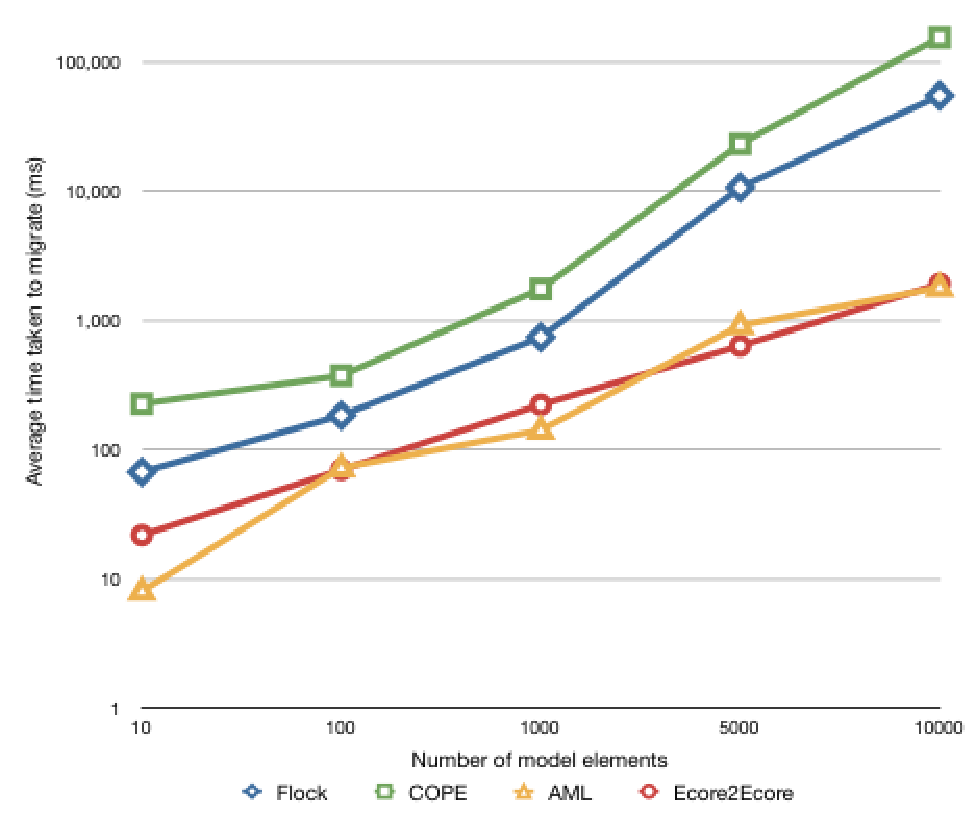
\includegraphics[width=10cm]{6.Evaluation/images/migration_tool_performance.pdf}
	\caption{Migration tool performance comparison.}
	\label{fig:performance}
\end{figure}

To measure performance, five sets of Petri net models were generated at random. Models in each set contained 10, 100, 1000, 5,000, and 10,000 model elements.  Figure~\ref{fig:performance} shows the average time taken by each tool to execute migration across 10 repetitions for models of different sizes. Note that the Y axis has a logarithmic scale. The results indicate that, for the Petri nets co-evolution example, AML and Ecore2Ecore execute migration significantly more quickly than COPE and Flock, particularly when the model to be migrated contains more than 1,000 model elements. Figure~\ref{fig:performance} indicates that, for the Petri nets co-evolution example, Flock executes migration between two and three times faster than COPE, although the author of COPE reports that turning off validation causes COPE to perform similarly to Flock.


\subsection{Discussion}
\label{sec:discussion}
The comparison described above highlights similarities and differences between a representative sample of model migration approaches. From this comparison, guidance for selecting between tools was synthesised. The guidance is presented below, and was produced by all four participants in the comparison (Herrmannsd\"{o}erfer, Williams, Kolovos and the author). 

COPE captures co-evolution patterns (which apply to both model and metamodel), while Ecore2Ecore, AML and Flock capture only model migration patterns (which apply just to models). Because of this, COPE facilitates a greater degree of re-use in model migration than other approaches. However, the order in which the user applies patterns with COPE impacts on both metamodel evolution and model migration, which can complicate pattern selection particularly when a large amount of evolution occurs at once. The re-usable co-evolution patterns in COPE make it well suited to migration problems in which metamodel evolution is frequent and in small steps.

Flock, AML and Ecore2Ecore are preferable to COPE when metamodel evolution has occurred before the selection of a migration approach. Because of its use of co-evolution patterns, we conclude that COPE is better suited to forward- rather than reverse-engineering.

Through its Convergence View and integration with the EMF metamodel editor, COPE facilitates metamodel analysis that is not possible with the other approaches considered in this paper. COPE is well-suited to situations in which measuring and reasoning about co-evolution is important.

In situations where migration involves modelling technologies other than EMF, AML and Flock are preferable to COPE and Ecore2Ecore. AML can be used with models represented in KM3, while Flock can be used with models represented in MDR, XML and CZT. Via the connectivity layer of Epsilon, Flock can be extended to support further modelling technologies.

There are situations in which Ecore2Ecore or AML might be preferable to Flock and COPE. For large models, Ecore2Ecore and AML might execute migration significantly more quickly than Flock and COPE. Ecore2Ecore is the only tool that has no technical dependencies (other than a modelling framework). In situations where migration must be embedded in another tool, Ecore2Ecore offers a smaller footprint than other migration approaches. Compared to the other approaches considered in this paper, AML automatically generates migration strategies with the least guidance from the user.

Despite these advantages, Ecore2Ecore and AML are unsuitable for some types of migration problem, because they are less expressive than Flock and COPE. Specifically, changes to the containment of model elements typically cannot be expressed with Ecore2Ecore and changes that are classified by %\cite{gruschko07towards} as \emph{breaking and non-resolvable}
\cite{herrmannsdoerfer08automatability} as \emph{metamodel-specific}
cannot be expressed with AML. Because of this, it is important to investigate metamodel changes before selecting a migration tool. Furthermore, it might be necessary to anticipate which types of metamodel change are likely to arise before selecting a migration tool. Investing in one tool to discover later that it is no longer suitable causes wasted effort.

\begin{table}[hbtp]
	\centering
	\begin{tabular}{|c|c|}
	\hline
	\textbf{Requirement}    & \textbf{Recommended Tools} \\
	\hline
	Frequent, incremental co-evolution                & COPE \\
	\hline
	Reverse-engineering                               & AML, Ecore2Ecore, Flock \\
	\hline
	Modelling technology diversity                    & Flock \\
	\hline
	Quicker migration for larger models               & AML, Ecore2 Ecore \\
	\hline
	Minimal dependencies                              & Ecore2Ecore \\
	\hline
	Minimal hand-written code                         & AML, COPE \\
	\hline
	Minimal guidance from user                        & AML \\
	\hline
	Support for metamodel-specific migrations   & COPE, Flock \\
%	Support for breaking and non-resolvable changes   & COPE, Flock \\
	\hline
	\end{tabular}
	\caption[Summary of tool selection advice]{Summary of tool selection advice. (Tools are ordered alphabetically).}
	\label{tab:advice}
\end{table}

\subsubsection{Strengths and Weaknesses of Flock}
The comparison and guidance highlight strengths and weaknesses of AML, COPE, Ecore2Ecore and Flock. The findings for Flock are now summarised.

\paragraph{Strengths} Flock was the only co-evolution tool suitable for performing model migration when the original and evolved metamodels are specified in different modelling technologies. AML, Ecore2Ecore and COPE are interoperable with a single modelling technology, the Eclipse Modelling Framework. Migrating models between metamodels represented in different modelling technologies would require modification of the co-evolution tool when using AML, Ecore2Ecore or COPE and hence, model migration with Flock requires less effort than using AML, Ecore2Ecore or COPE when migrating between modelling technologies. This was a key requirement for the co-evolution example described in the sequel.

For the examples of metamodel evolution explored here, Flock (and COPE) is more expressive than AML, but requires more guidance from the user. This is consistent with the trade-off between flexibility and level of automation of co-evolution approaches identified in Chapter~\ref{Analysis}.

Unlike COPE, Flock (and AML and Ecore2Ecore) does not make assumptions on the way i which metamodel evolution will be specified. With Flock, AML and Ecore2Ecore, metamodel evolution need not occur at the same time or in the same development environment as the formulation of the model migration strategy. For this reason, Flock (and AML and Ecore2Ecore) arguably lead to more productive model migration when used to formulate a model migration strategy after metamodel evolution has already been specified, as was the case for the GMF Graph example used in this section.

\paragraph{Weaknesses} The results presented here indicate that model migration with Flock takes longer to execute than with AML and Ecore2Ecore. This is likely because Flock migration strategies are interpreted, while AML and Ecore2Ecore migration strategies are compiled. A compiler for Flock would likely increase execution time, but, at present, Epsilon, the platform atop which Flock is built, lacks the infrastructure required for constructing compilers. As such, model migration with Flock is likely to be less productive than with AML or Ecore2Ecore when a large models or a large number of models are to be migrated.

Compared to COPE and AML, Flock lacks re-use of model migration patterns across varying metamodels. In Flock, model migration is specified in terms of concrete metamodel types and cannot be re-used for different metamodels. By contrast, COPE and AML capture model migration in a metamodel-independent manner. When migration is likely to be a commonly occurring practice, the use of COPE or AML rather than Flock is likely to led to increased productivity and understandability of model migration, because the metamodel-independent migration patterns will likely increase re-use and provide a vocabulary for describing migration. Section~\ref{sec:future_work} describes ways in which Flock might be extended to capture metamodel-independent migration patterns.

\subsection{Summary}
The work presented in this section compared a representative sample of approaches to automating developer-driven co-evolution using an expert evaluation. The comparison was performed by following a methodical process and using an example from a real-world MDE project. Some preliminary recommendations and guidelines in choosing a co-evolution tool were synthesised from the presented results and are summarised in Table~\ref{tab:advice}. The comparison was carried out by the tool developers (or stand-ins where the developers were unable to participate fully). Each developer used a tool other than their own so that the comparison could more closely emulate the level of expertise of a typical user.

The results of the comparison suggested situations in which the use of Flock might lead to increased productivity and understandability of model migration, and, conversely, situations in which an alternative tool might be preferable. The comparison results suggest that Flock is well-suited to co-evolution when models are to be migrated between different modelling technologies, when migration involves metamodel-specific detail, and when metamodel evolution has occurred prior to -- or in a different development environment to -- the formulation of a model migration strategy. Additionally, Flock might be improved via optimisations to increase the execution time of large models or a large number of models, and by considering the ways in which model migration patterns could be captured in a metamodel-independent manner.

Some criteria were excluded from the comparison because of the method employed. For instance, the learnability of a tool affects the productivity of users, and, as such, affects tool selection. However, drawing conclusions about learnability (and also productivity and usability) is challenging with the comparison method employed because of the subjective nature of these characteristics. A comprehensive user study (with hundreds of users) would be more suitable for assessing these types of criteria.
